\documentclass[tikz]{standalone}
\usepackage{pgfplots}
\pgfplotsset{compat=1.16}
\pgfplotsset{
    no markers,
    axis lines=middle,
    xtick={\empty},
    ytick={\empty},
    every axis/.style={
        scale only axis,
        unit vector ratio*=1 1 1,
    },
    every axis plot/.append style={ultra thick},
    xlabel style={at={(ticklabel* cs:1)}, anchor=north west},
    ylabel style={at={(ticklabel* cs:1)}, anchor=east},
}

\def\vgamma{0.75}

\begin{document}
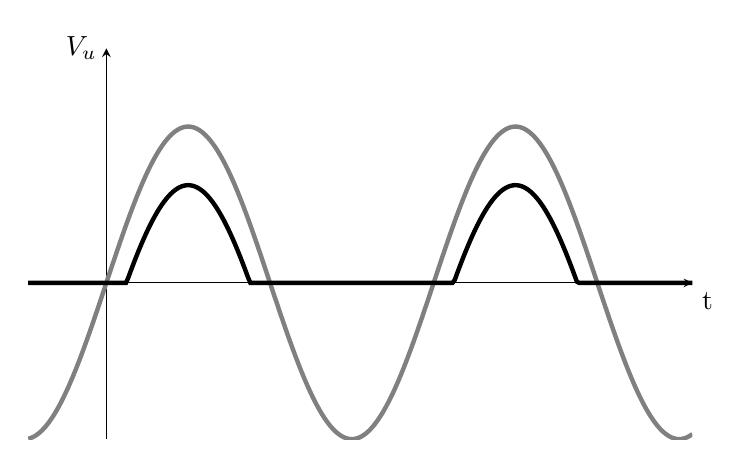
\begin{tikzpicture}[
    declare function={
        func(\x) = (\x > \vgamma) * (\x - \vgamma);
    }]
    \begin{axis}[xlabel=t, ylabel=$V_u$,
                ymin=-2,
                xmin=-1,
                xmax=7.5,
                ymax=3]

        \addplot[gray, samples=300, domain=-1:7.5]{
            2*sin(1.5*deg(x))
        };

        \addplot[samples=300, domain=-1:7.5]{
            func(2*sin(1.5*deg(x)))
        };
    \end{axis}
\end{tikzpicture}
\end{document}
